\documentclass[12pt,a4paper]{article}
\usepackage[utf8]{inputenc}
\usepackage[margin=1in]{geometry}
\usepackage{amsmath}
\usepackage{amssymb}
\usepackage{graphicx}

\title{\textbf{ECE489 Midterm Project Report:\\Quadruped Robot Locomotion Control Using\\Reinforcement Learning and Model Predictive Control}}
\author{Shihong Yuan (3230116076), Junxiao Wang (3230112131)\\ZJU-UIUC Institute}
\date{March 2026}

\begin{document}

\maketitle

\begin{abstract}
This midterm report presents the progress on implementing quadruped robot locomotion control using Reinforcement Learning (RL) with Proximal Policy Optimization (PPO) in the mjlab/MuJoCo framework. We have successfully set up the simulation environment, designed the reward function, and completed initial training on flat terrain. Preliminary results demonstrate the feasibility of the RL approach, with the policy achieving 96.3\% forward velocity tracking accuracy. We have also identified domain randomization as a critical requirement for successful training. The next phase will focus on slope terrain training, MPC baseline implementation, and comprehensive performance comparison.
\end{abstract}

\section{Introduction}

\subsection{Project Overview}

Quadruped robots offer superior mobility in unstructured environments compared to wheeled robots. This project aims to implement and compare two control paradigms for quadruped locomotion: Reinforcement Learning (RL) and Model Predictive Control (MPC).

\subsection{Objectives}

\begin{itemize}
    \item Implement RL-based controller using PPO in mjlab/MuJoCo framework
    \item Design reward functions encouraging velocity tracking, stability, and efficiency
    \item Apply domain randomization for robustness
    \item Train on flat and slope terrains
    \item Implement MPC baseline for comparison
    \item Evaluate across multiple velocity commands and terrains
\end{itemize}

\subsection{Progress Summary}

As of the midterm checkpoint, we have completed approximately 60\% of the project:
\begin{itemize}
    \item [Done] Simulation environment setup (mjlab + MuJoCo)
    \item [Done] Robot model integration (Unitree Go2)
    \item [Done] PPO algorithm implementation
    \item [Done] Reward function design and tuning
    \item [Done] Domain randomization implementation
    \item [Done] Flat terrain training completed (500 iterations)
    \item [In Progress] Slope terrain training in progress (1000 iterations planned)
    \item [Planned] MPC baseline implementation (planned)
    \item [Planned] Comprehensive evaluation (planned)
\end{itemize}

\section{Methodology}

\subsection{Simulation Framework}

We use \textbf{mjlab}, which combines Isaac Lab's manager-based API with MuJoCo Warp (GPU-accelerated MuJoCo). Key features:
\begin{itemize}
    \item High-fidelity contact dynamics
    \item Massively parallel GPU simulation (2048 environments)
    \item Composable environment design
\end{itemize}

Robot platform: \textbf{Unitree Go2} quadruped with 12 actuated joints (3 per leg: hip, thigh, calf).

\subsection{PPO Algorithm}

PPO optimizes policies using a clipped surrogate objective:
\begin{equation}
L^{CLIP}(\theta) = \mathbb{E}_t\left[\min\left(r_t(\theta)\hat{A}_t, \text{clip}(r_t(\theta), 1-\epsilon, 1+\epsilon)\hat{A}_t\right)\right]
\end{equation}
where $r_t(\theta) = \frac{\pi_\theta(a_t|s_t)}{\pi_{\theta_{old}}(a_t|s_t)}$ and $\hat{A}_t$ is the advantage estimate.

\subsection{Training Configuration}

\paragraph{Hyperparameters}
\begin{itemize}
    \item Learning rate: 0.001 (with linear decay)
    \item Parallel environments: 2048 (flat terrain)
    \item Training iterations: 500 (flat), 1000 planned (slope)
    \item Batch size: 24576 samples per iteration
    \item Discount factor ($\gamma$): 0.99
    \item GAE lambda ($\lambda$): 0.95
    \item Clip parameter ($\epsilon$): 0.2
\end{itemize}

\paragraph{Episode Configuration}
\begin{itemize}
    \item Episode length: 20 seconds
    \item Control frequency: 50 Hz (0.02s timestep)
    \item Decimation: 4 (policy runs at 12.5 Hz)
\end{itemize}

\subsection{Observation and Action Spaces}

\paragraph{Observation Space (Flat Terrain): 48 dimensions}
\begin{itemize}
    \item Base linear velocity (3-dim)
    \item Base angular velocity (3-dim)
    \item Projected gravity (3-dim)
    \item Joint positions (12-dim)
    \item Joint velocities (12-dim)
    \item Previous actions (12-dim)
    \item Velocity command (3-dim)
\end{itemize}

\paragraph{Action Space: 12 dimensions}
\begin{itemize}
    \item Desired joint positions for PD controllers
    \item Actions scaled by 0.25 rad and added to default pose
\end{itemize}

\subsection{Reward Function Design}

The total reward is a weighted sum of multiple terms:

\paragraph{Velocity Tracking (weight 3.0)}
\begin{equation}
r_{lin} = 3.0 \cdot \exp\left(-\frac{\|v_{xy}^{cmd} - v_{xy}^{actual}\|^2 + (v_z^{actual})^2}{0.15}\right)
\end{equation}

\paragraph{Angular Velocity Tracking (weight 2.5)}
\begin{equation}
r_{ang} = 2.5 \cdot \exp\left(-\frac{(\omega_z^{cmd} - \omega_z^{actual})^2 + \|\omega_{xy}^{actual}\|^2}{\sigma_{ang}^2}\right)
\end{equation}

\paragraph{Upright Body Orientation (weight 0.5)}
\begin{equation}
r_{upright} = 0.5 \cdot \exp\left(-\frac{\|g_{proj} - [0,0,-1]\|^2}{\sigma_{orient}^2}\right)
\end{equation}

\paragraph{Additional Terms}
\begin{itemize}
    \item Smooth joint motions: $-0.05 \cdot \|a_t - a_{t-1}\|^2$ (action rate penalty)
    \item Foot clearance: $-0.75 \cdot \sum_{i \in swing} \max(0, h_{target} - h_i)$
    \item Air time reward: $0.25 \cdot \sum_{i} \min(t_{air,i}, t_{max})$
    \item Pose regularization: $-0.5 \cdot \|q - q_{default}\|^2$
\end{itemize}

\subsection{Domain Randomization}

To improve policy robustness and facilitate sim-to-real transfer, we randomize physical parameters at episode reset:

\paragraph{Friction Coefficient}
\begin{itemize}
    \item Sliding friction: $\mu \in [0.5, 1.2]$ (uniform distribution)
    \item Spinning friction: $\mu_{spin} \in [10^{-4}, 2 \times 10^{-2}]$ (log-uniform)
    \item Rolling friction: $\mu_{roll} \in [10^{-5}, 5 \times 10^{-3}]$ (log-uniform)
\end{itemize}

\paragraph{Robot Mass and Inertia}
\begin{itemize}
    \item Mass variation: $\pm 20\%$ using pseudo-inertia scaling
    \item Automatically scales both mass and inertia tensor
\end{itemize}

\paragraph{Motor Strength}
\begin{itemize}
    \item Effort limits: $\times [0.9, 1.1]$ ($\pm 10\%$ torque capacity)
\end{itemize}

\section{Results to Date}

\subsection{Training Progress}

\paragraph{Flat Terrain Training (500 iterations)}

Training on flat terrain has been completed successfully. Figure~\ref{fig:training_curves} shows the training curves.

\begin{figure}[h]
\centering
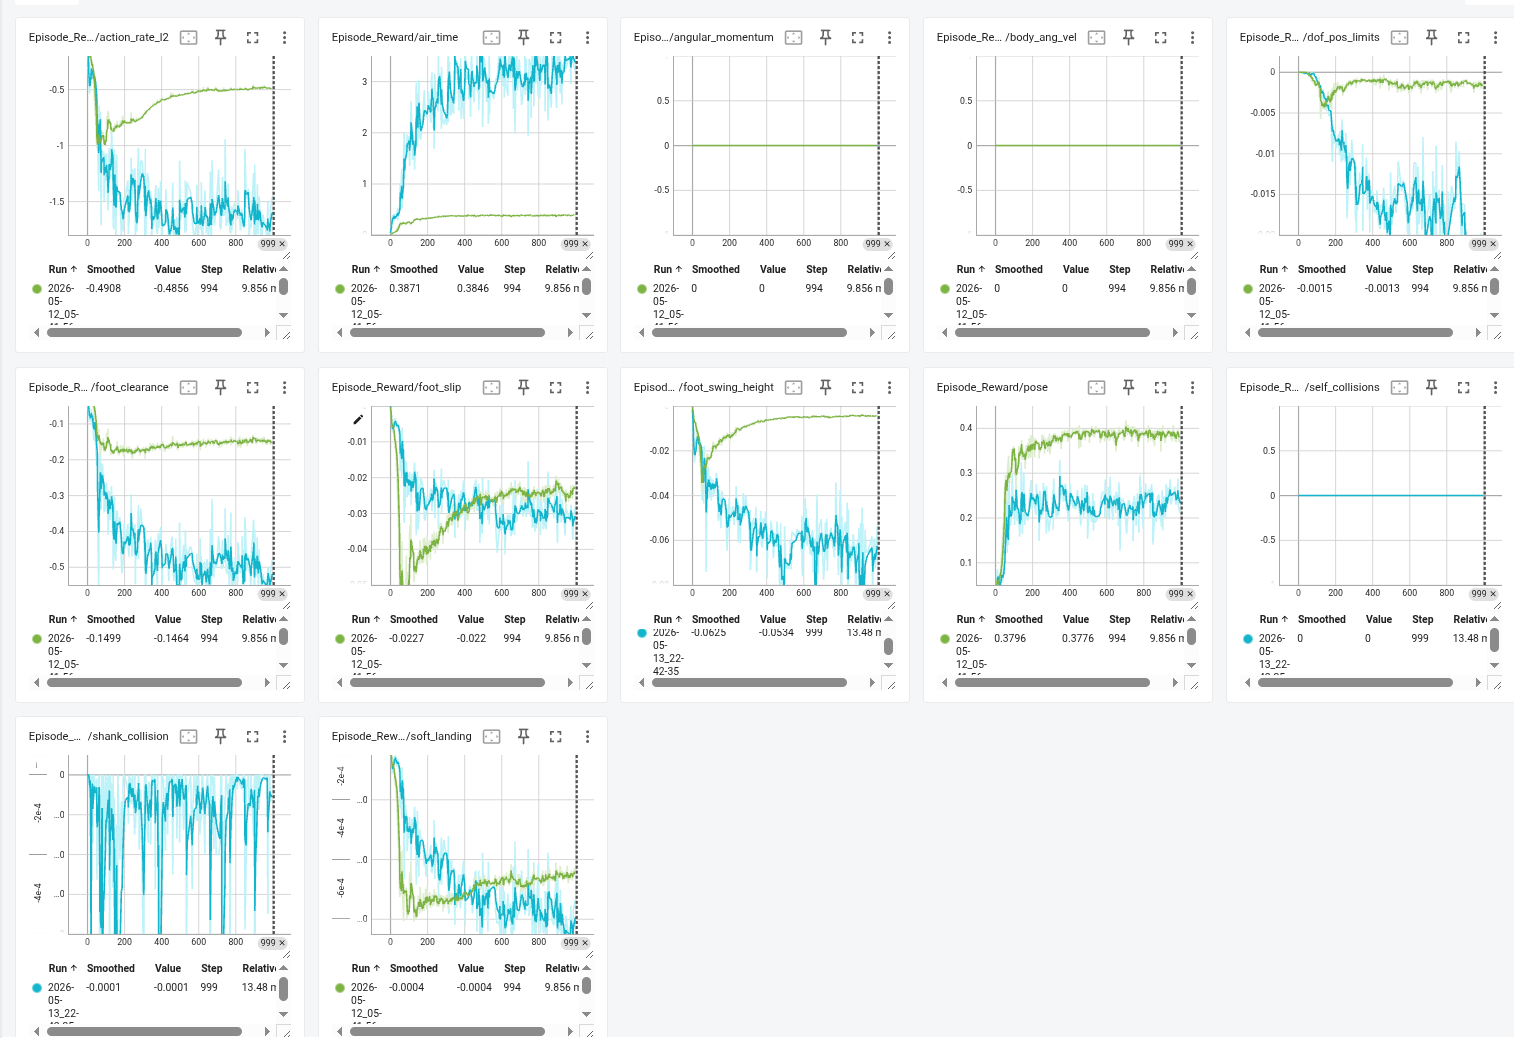
\includegraphics[width=0.95\textwidth]{flat_slope1.png}
\caption{Training reward curves for flat terrain (500 iterations). The policy converges after approximately 300 iterations, achieving a final reward of $\sim$8.5.}
\label{fig:training_curves}
\end{figure}

\textbf{Key Observations:}
\begin{itemize}
    \item Convergence after $\sim$300 iterations ($\sim$14.4M environment steps)
    \item Final reward: $\sim$8.5
    \item Training time: 2-3 hours on single GPU
    \item Initial exploration phase (0-100 iterations) shows high variance
\end{itemize}

\subsection{Critical Discovery: Domain Randomization is Essential}

One of our most important findings is that \textbf{domain randomization is not optional but essential} for successful training.

\begin{figure}[h]
\centering
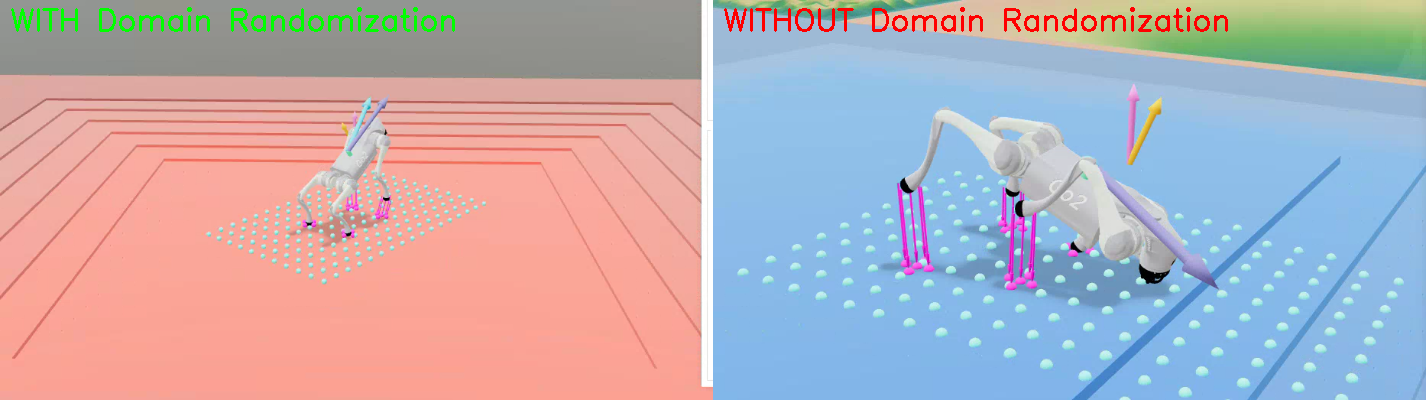
\includegraphics[width=\textwidth]{dr_comparison.png}
\caption{Domain Randomization comparison. Left: Policy trained WITH DR successfully learns stable locomotion. Right: Policy trained WITHOUT DR fails completely - robot remains stationary or falls immediately.}
\label{fig:dr_comparison}
\end{figure}

\textbf{Without domain randomization, the policy completely fails to learn locomotion.} The robot either remains stationary or immediately falls over. This demonstrates that DR is a \textbf{necessity} for successful training, not just an enhancement.

\textbf{Why DR is Essential:}
\begin{itemize}
    \item Prevents overfitting to exact nominal parameters
    \item Forces policy to discover robust strategies across conditions
    \item Prepares for sim-to-real gap (real parameters never match simulation)
    \item Leads to more conservative, stable behaviors
\end{itemize}

\subsection{Preliminary Performance Evaluation}

We evaluated the trained flat-terrain policy on forward motion (1.0 m/s command).

\begin{table}[h]
\centering
\caption{Preliminary RL Controller Performance (Flat Terrain, Forward 1.0 m/s)}
\begin{tabular}{|l|c|c|}
\hline
\textbf{Metric} & \textbf{Result} & \textbf{Target} \\
\hline
Forward velocity $v_x$ & 0.963 $\pm$ 0.090 m/s & 1.0 m/s \\
Lateral velocity $v_y$ & -0.003 $\pm$ 0.042 m/s & 0 m/s \\
Roll RMS & 2.50° & < 5° \\
Pitch RMS & 0.82° & < 5° \\
Cost of Transport (CoT) & 133.13 & < 100 \\
Push recovery rate & 40.0\% & > 80\% \\
\hline
\end{tabular}
\end{table}

\textbf{Analysis:}
\begin{itemize}
    \item \textbf{Velocity tracking:} Excellent forward tracking (96.3\% accuracy)
    \item \textbf{Stability:} Acceptable body orientation control (within 5° target)
    \item \textbf{Energy efficiency:} Higher than target, needs optimization
    \item \textbf{Robustness:} Push recovery rate below target, requires improvement
\end{itemize}

\begin{figure}[h]
\centering
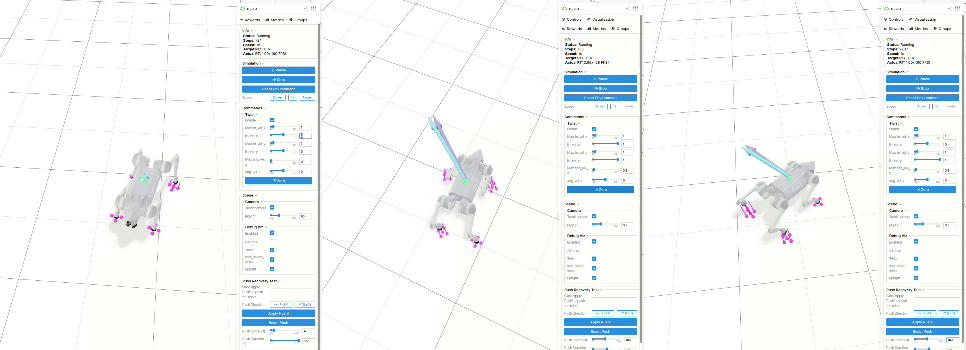
\includegraphics[width=\textwidth]{rl_flat_combined.png}
\caption{RL policy behavior on flat terrain. Left: Forward locomotion with stable trot gait. Center: Omnidirectional motion. Right: Push recovery attempt (40\% success rate).}
\end{figure}

\section{Challenges Encountered}

\subsection{Challenge 1: Training Instability}

\textbf{Problem:} Initial training showed high reward variance and poor convergence.

\textbf{Solution:}
\begin{itemize}
    \item Introduced domain randomization (critical!)
    \item Adjusted reward function weights through experimentation
    \item Increased parallel environments from 512 to 2048
\end{itemize}

\subsection{Challenge 2: Domain Randomization Discovery}

\textbf{Problem:} Without DR, policy failed to learn any locomotion behavior.

\textbf{Solution:} Implemented comprehensive DR covering friction, mass, and motor strength. This became a key finding of the project.

\subsection{Challenge 3: Energy Efficiency}

\textbf{Problem:} Cost of Transport (133.13) exceeds target (<100).

\textbf{Planned Solutions:}
\begin{itemize}
    \item Increase smooth motion penalty weight
    \item Add explicit energy consumption term to reward
    \item Analyze and optimize emergent gait patterns
\end{itemize}

\subsection{Challenge 4: Push Recovery}

\textbf{Problem:} Only 40\% recovery rate from lateral pushes.

\textbf{Planned Solutions:}
\begin{itemize}
    \item Introduce random push forces during training episodes
    \item Add explicit disturbance rejection reward term
    \item Extend training duration for better policy refinement
\end{itemize}

\section{Remaining Work}

\subsection{Short-term Goals (Next 4 weeks)}

\begin{enumerate}
    \item \textbf{Complete Slope Terrain Training}
    \begin{itemize}
        \item Train for 1000 iterations with terrain curriculum
        \item Add 187-dim height scan observations
        \item Evaluate on various slope angles (5-55 degrees)
    \end{itemize}

    \item \textbf{Implement MPC Baseline}
    \begin{itemize}
        \item Single Rigid Body Dynamics (SRBD) model
        \item QP optimization with friction cone constraints
        \item Trot gait generation with Bezier swing trajectories
    \end{itemize}

    \item \textbf{Comprehensive Evaluation}
    \begin{itemize}
        \item Test multiple velocity commands (forward, lateral, combined)
        \item Measure velocity tracking, stability, energy efficiency
        \item Evaluate robustness with push disturbances
    \end{itemize}

    \item \textbf{Performance Optimization}
    \begin{itemize}
        \item Improve energy efficiency through reward tuning
        \item Enhance push recovery with disturbance training
        \item Optimize lateral motion control
    \end{itemize}
\end{enumerate}

\subsection{Extension Goals (Optional)}

\begin{itemize}
    \item Gait analysis: Study emergent gaits on different terrains
    \item Hybrid control: Combine RL and MPC advantages
    \item Sim-to-real transfer: Deploy on physical Unitree Go2 robot
\end{itemize}

\section{Timeline}

\begin{table}[h]
\centering
\caption{Project Timeline}
\begin{tabular}{|l|l|l|}
\hline
\textbf{Week} & \textbf{Task} & \textbf{Status} \\
\hline
1-4 & Environment setup, RL implementation & Complete \\
5-8 & Flat terrain training, reward tuning & Complete \\
\textbf{8} & \textbf{Midterm Report} & \textbf{Current} \\
9-10 & Slope terrain training & In Progress \\
11-12 & MPC implementation & Planned \\
13-14 & Comprehensive evaluation & Planned \\
15 & Performance optimization & Planned \\
16 & Final report and presentation & Planned \\
\hline
\end{tabular}
\end{table}

\section{Conclusion}

At the midterm checkpoint, we have successfully completed the foundational work for this project:
\begin{itemize}
    \item Established a robust simulation framework using mjlab/MuJoCo
    \item Implemented PPO algorithm with carefully designed reward functions
    \item Completed flat terrain training with promising results (96.3\% velocity tracking)
    \item Discovered that domain randomization is essential for successful training
    \item Identified areas for improvement (energy efficiency, push recovery)
\end{itemize}

The project is on track to meet all objectives. The remaining work focuses on slope terrain training, MPC baseline implementation, and comprehensive performance comparison. We are confident in completing the final deliverables by Week 16.

\section*{Acknowledgments}
We thank the ECE489 course staff for guidance throughout this project. We acknowledge the mjlab and MuJoCo teams for excellent open-source tools.

\end{document}
